\subsection{Явление Мандельштама-Бриллюэна}


Рассмотрим случай слабой неоднородности для уравнений относительно $\vc{H}$ и $\vc{E}'$:
\begin{align*}
    &\rot \vc{H}' - \frac{\varepsilon_0}{c}\frac{\partial \vc{E}'}{\partial t} = \frac{4\pi}{c} \frac{\partial }{\partial t} \delta \vc{P},
    &\div(\varepsilon_0 \vc{E}') = - 4 \pi \div (\delta \vc{P}), \\
    &\rot \vc{E}' - \frac{1}{c} \frac{\partial \vc{H}'}{\partial t} =0,
    &\div \vc{H}' = 0,
\end{align*}
где $\delta \vc{P} = \frac{\delta \varepsilon}{4 \pi} \vc{E}_0$. 
Эти уравнения линейный и однородны как относительно полей, так и относительно $\delta \varepsilon$. Отсюда следует, что если представить $\delta \varepsilon$ в виде $\delta \varepsilon = \sum \delta_i \varepsilon$, то в линейном приближении можем рассеянное излучение может быть получено суперпозицией полей, рассейяных одной неоднородностью. 

Рассмотрим случай, когда $\delta \varepsilon = a \exp\left(-i \vc{K} \cdot \vc{r}\right)$, где $a$ и $\vc{K}$ -- постоянные. Представляя падающую волну, как плоскую
\begin{equation*}
    \vc{E}_0 = \vc{A} e^{i(\omega t - \smallvc{k} \smallvc{r})},
    \hspace{5 mm} 
    \vc{H}_0 = \vc{B} e^{i(\omega t -\smallvc{k} \smallvc{r})}.
\end{equation*}
Разобьеё среду плоскостями с расстоянием $\Lambda = \frac{2\pi}{K}$, тогда фазы вторичных источников будут одинаковы (рис. \ref{fig:ggg}). 
\begin{figure}[h]
    \centering
    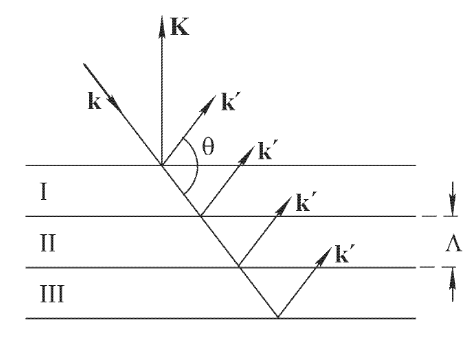
\includegraphics[width=0.25\textwidth]{figures/ggg.png}
    \caption{Иллюстраия к явлению Мандельштама-Бриллюэна}
    \label{fig:ggg}
\end{figure}
Чтобы источники не гасили, а усиливали друг друга, необходимо выполнение \textit{условия Брэгга-Вульфа}:
\begin{equation*}
    2 \Lambda \sin(\theta/2) = m \lambda,
\end{equation*}
где $\theta$ -- угол рассеяния, а $m$ -- порядок дифракционного спектра. 

Покажем, что $m=1$. Все плоские, отраженные различными слоями, сложатся в волну $\vc{E}' = \vc{A}' e^{i(\omega t 0 \smallvc{k}' \cdot \smallvc{r}')}$, где волновой вектор $\vc{k}'$ определяет направление распространения отраженных волн. С другой стороны, дополнительная поляризация среды
\begin{equation*}
    \delta \vc{P} = \frac{\vc{E}_0}{4 \pi} \delta \varepsilon = \frac{a \vc{A}}{4 \pi} e^{i[\omega t - \left(\smallvc{k}+\smallvc{K}\right)\smallvc{r}]}.
\end{equation*}
Подставляя эти выражения во второе уравнение и сравнивая показатели, получаем $\vc{k} - \vc{k} = \vc{K}$, откуда
\begin{equation*}
    2 \Lambda \sin(\theta/2) = \lambda,
\end{equation*}
таким образом на синусоидальной неоднородности диэлектрической проницаемости в линейном приближении получается дифракционный спектр \textit{только первого порядка}. 

Любую неоднродность в среде можно по Фурье представить в виде суперпозиции плоских синусоидальных неоднородностей различных направлений. Они рассеивают свет \textit{незаивисимо} друг от друга, но при фиксированном направлении эффективны только неоднородности,  волновой вектор $\vc{K}$ которых направлен по \textit{биссектрисе угла, дополнительного к $\theta$ до $\pi$}.



Учтём $\delta \varepsilon \equiv \delta \varepsilon(t)$, считая $\varepsilon \equiv \varepsilon(\rho)$, запишем $\Delta \varepsilon = (d\varepsilon/d \rho) \Delta \rho$, где $\rho$ -- плотность.  Всякая неоднородность плотности в среде -- \textit{источник звуковых волн}. Разложим $\Delta \rho$ в интеграл Фурье и возьмём только те гармоники, которые существенны для рассеяния волн в рассматриваемом направлении, $\vc{K}$ которых определен выше, которому соответсвует определенная $\Omega$ и направления распространения звуковой волны: $\upuparrows \vc{K}$ и $\downdownarrows \vc{K}$. Тогда $\delta \varepsilon$ представляется суммой
\begin{equation*}
    \delta \varepsilon = \delta \varepsilon_1 + \delta \varepsilon_2,
    \hspace{5 mm} 
    \delta \varepsilon_1 = a_1 e^{i(\Omega t - \smallvc{K} \cdot \smallvc{r})},
    \hspace{5 mm} 
    \delta \varepsilon_2 = a_2 e^{i(\Omega t + \smallvc{K} \cdot \smallvc{r})}.
\end{equation*}
Им соответсвуют вектор дополнительной поляризации среды
\begin{align*}
    \delta \vc{P}_1 &= \frac{\vc{E}_0}{4 \pi} \delta \varepsilon_1 = \frac{a_1 \vc{A}}{4 \pi} e^{i[(\omega + \Omega)t - (\smallvc{k}+\smallvc{K})\cdot \vc{r}]}, \\
    \delta \vc{P}_2 &= \frac{a_2 \vc{A}}{4 \pi} e^{i[(\omega-\Omega)t - (\smallvc{k}+\smallvc{K})\cdot \smallvc{r}]}.
\end{align*}
Таким образом рассеянное излучение будет происходить с частотами $\omega + \Omega$ и $\omega - \Omega$ (модуляция световой волны акустической волны). Это явление называется \textit{тонкой структурой линий рэлевского рассеяния} или \textit{рассеянием Мандельштама-Бриллюэна}. Смещение частоты $\Omega = K v = (2\pi/\Lambda) v$, где $v$ -- скорость звука, а $\Lambda$ -- длина звукоыой волны. Итого, можем записать
\begin{equation*}
    \Omega = \frac{4 \pi v}{\lambda} \sin \frac{\theta}{2} = 2 \omega n \frac{v}{c} \sin \frac{\theta}{2},
\end{equation*}
где $c$ -- скорость света в вакууме, а $n$ -- показатель преломления среды. 



Иная трактовка дублета Мандельштама-Бриллюэна -- \textit{доплеровское изменение частоты света} при отражении от аккустической волны. Доплеровское изменение частоты определяется формулой
\begin{equation*}
    \frac{\Omega}{\omega} = \frac{2 v \sin \theta/2}{c/n},
\end{equation*}
что соответсвует предыдущему соотношению. 



Забавный факт про жидкости: там в рассеянном свете есть несмещенная компонента, всё потому, что
\begin{equation*}
    \delta V = (\partial_P V)_S \delta P + (\partial_S V)_P \delta S,
\end{equation*}
то есть флуктуации объема обусловлены не только флуктуациями давления, но и флутуациями энтропии, второе и вызывает \textit{несмещенную компоненту}. 




\textbf{Нелинейный эффект}. Рассмотрим мощный световой импульс, генерирующем давление
\begin{equation*}
    \mathcal P = \frac{1}{8 \pi} \left(\rho \frac{d \varepsilon}{d \rho} \right)E^2,
\end{equation*}
где $\rho d_\rho \varepsilon \sim 1$, соответсвенно $\mathcal P$ может достигать $10^5$ атм, а тогда световые и оптические волны надо рассматривать \textit{совместно}. Они описываются сложной охапкой нелинейный диффуров из электродинамики и акустики, что генерирует целый пучок разных эффектов, \textit{вынужденное рассеяние рассеяние Мандельштама-Бриллюэна}. 


Пусть, 
\begin{align*}
    \vc{E}_0 &= \vc{A}_0 \cos (\omega t - \vc{k}  \vc{r}), \\
    \vc{E}_1 &= \vc{A}_1 \cos \left[(\omega + \Omega) t - \vc{k}' \vc{r}\right], \\
    \vc{E}_2 &= \vc{A}_2 \cos\left[(\omega-\Omega)t - \vc{k}'\vc{r}\right], \\
    \vc{E}_3 &= \vc{A}_3 \cos[\omega t - \vc{k}' \vc{r}],
\end{align*}
-- напряженности электрического поля падающей и трех рассеянных волн Мандельштама-Бриллюэна. Последние три волны возникают при рассеянии на тепловых флуктуациях, интенсивности их малы, но давление определяется $(\vc{E}_0 + \vc{E}_1 + \vc{E}_2 + \vc{E}_3)^2$. Однако возбуждение звуковых волн связано только с низкочастотными членами, с косинусами разностных аргументов, вспоминая $\vc{K} = \vc{k}' - \vc{k}$, находим $\vc{A}_0 \vc{A}_1 \cos (\Omega t - \vc{K} \vc{r})$ -- волнуЮ распространяющуюся с той же фазой и в том же направлении, что и первичная звуковая волна из-за тепловых флуктуаций. Так будет происходить \textit{параметрическое усиление} акустической волны, и всех световых волн, на ней рассеянных. Это будет продолжаться до тех пор, пока интенсивность рассеянного света не станет сравнимой с интенсивностью падающего. Интересно, что \textit{вынуженное рассеяние Мандельштама-Бриллюэна когерентно}. 





